\begin{simulation}
\label{sim::jointlimit}
\end{simulation}

\noindent Considere o problema de rastreamento de posi��o (\nameref{traj1}) para o manipulador planar 3R da Figura \ref{fig::red} e uma fun��o $f$ para a $2^a$ junta, definida por ${q_{2d} = -1\,rad}$, $\zeta_2 = 0.5\,rad$, $\alpha_{f2} = 5$ e $k = 10$. Os resultados obtidos com o m�todo proposto para ${\boldsymbol \Gamma} = 5{\bf I}$ e ${\boldsymbol \Lambda}_p = 5{\bf I}$ s�o apresentados a seguir. 

\begin{figure}[!htp]
  		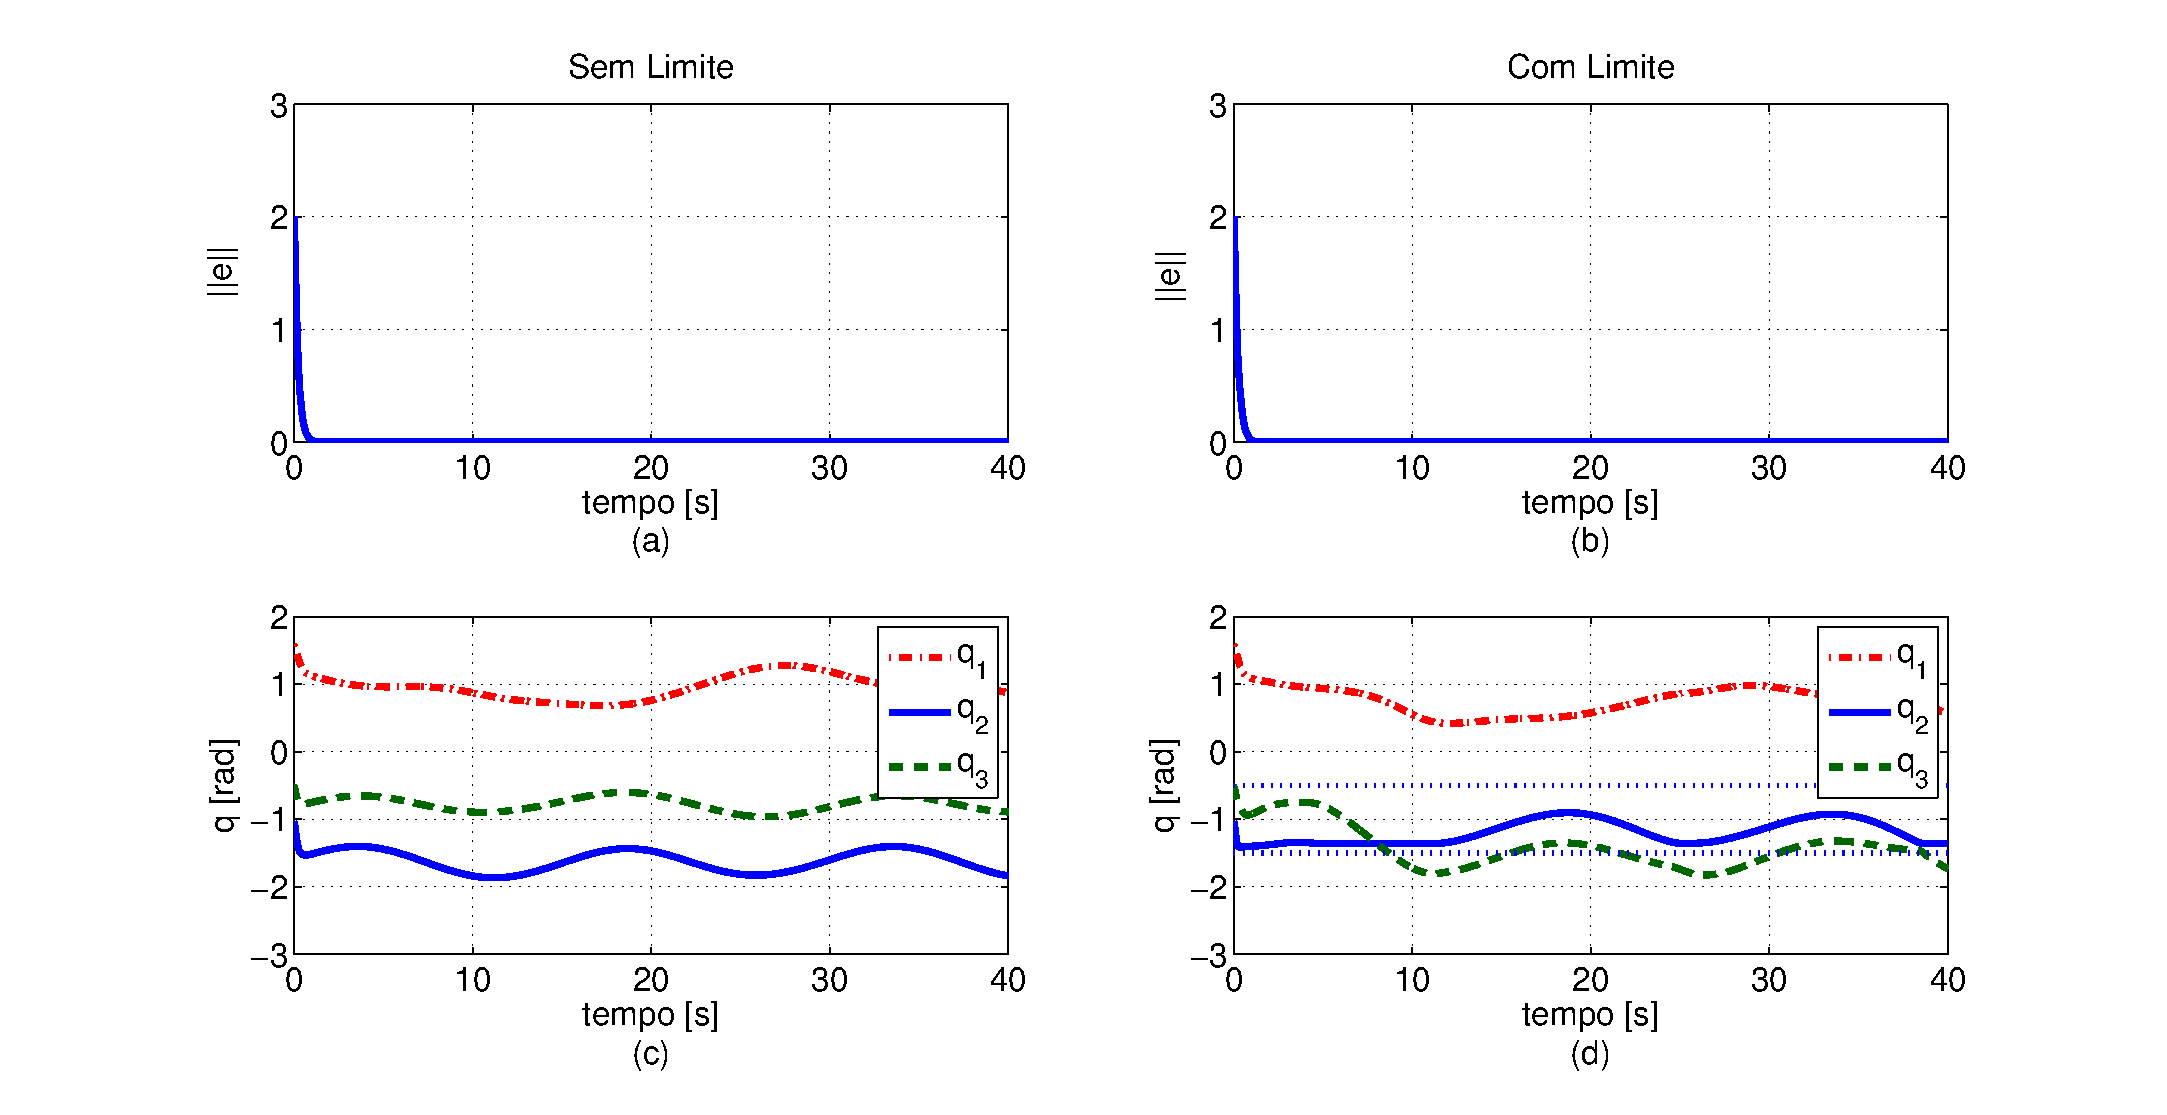
\includegraphics[trim = 1.7cm 1.7cm 4.4cm 0cm, scale = 0.46]{sim/junta_1.eps}\\ %\tiny{\,(b)} \\
\caption{Simula��o \ref{sim::jointlimit}: normas dos erros e �ngulos das juntas.}
\label{sim::jointlimit_1}
\end{figure}

A utiliza��o de $k = 10$ resulta em $f$ praticamente nula para $q_2 \in [q_{2d} - \zeta_2, q_{2d} + \zeta_2]$ e elevada para �ngulos fora desta faixa. Como visto na Figura \ref{sim::jointlimit_1}, o m�todo proposto permite manter o �ngulo da $2^a$ junta na faixa desejada com erro de rastreamento praticamente nulo para todo tempo $t$. Para a trajet�ria considerada, a redu��o de $\zeta_2$ torna o problema mais restrito e o rastreamento da posi��o se torna invi�vel sem que $f$ atinja valores elevados. A Figura \ref{sim::jointlimit_2} apresenta a norma do erro e as vari�veis de juntas obtidas para $\zeta_2 = 0.2\,rad$. Nota-se que o �ngulo da $2^a$ junta permanece na faixa definida, por�m s�o observados pequenos erros de rastreamento.

\begin{figure}[!htp]
  		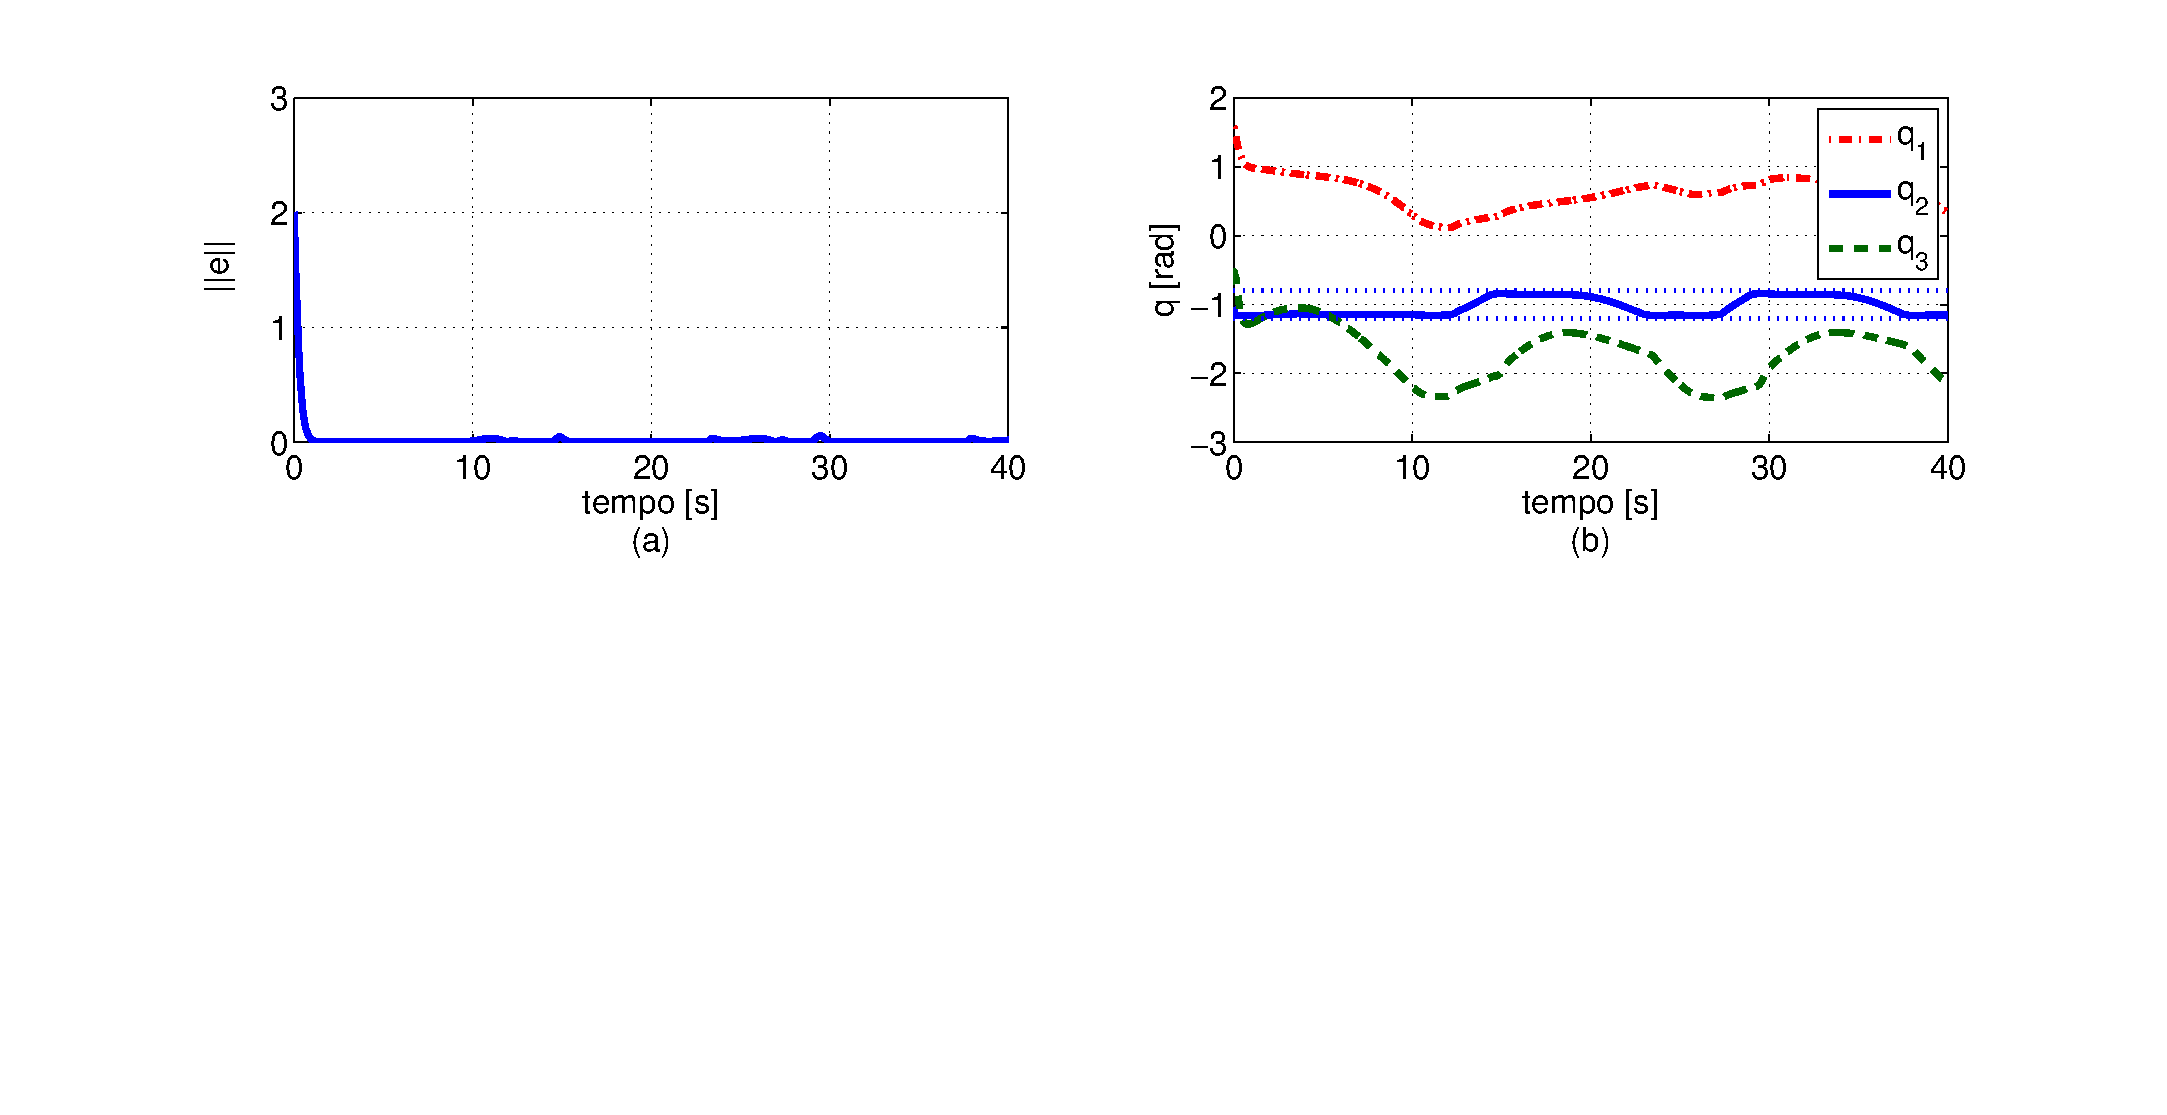
\includegraphics[trim = 1.7cm 10cm 4.4cm 0cm, scale = 0.46]{sim/junta_2.eps}\\ %\tiny{\,(b)} \\
\caption{Simula��o \ref{sim::jointlimit}: norma do erro e �ngulos das juntas para $\zeta_2 = 0.2\,rad$.}
\label{sim::jointlimit_2}
\end{figure}
